\documentclass[11pt, a4paper]{article}
\usepackage[utf8]{inputenc}
\usepackage[margin=1in]{geometry}
\usepackage{amsmath, amssymb, graphics, setspace}
\setlength\parindent{0pt}
\begin{document}

Quick tips before trying to solve the OLG model.
\begin{enumerate}
    \item Determine whether the zero steady state is possible: \\
    If $f(0) = 0$ (or, equivalently, $w(0) = 0$), then the zero (autarky) steady state exists.
    It may be stable or unstable, but it exists.
    \begin{itemize}
    \item Cobb-Douglas production function:\\
    $f(k) = k^\alpha \implies f(0) = 0$
    \item CES production function: \\
        \textbf{Important remark}: verify the exact functional form of the production function, in particular how the exponents are written.\\
        $f(k) = (\alpha k^\rho +(1-\alpha))^\frac{1}{\rho}$
        \begin{itemize}
            \item Complementary inputs ($\rho < 0$)\\
            $\lim_{k \rightarrow 0} f(k) = 0,$ assuming $\rho<0,\alpha \in (0,1).$ 
        \item Substitue inputs ($\rho > 0$)\\
            $\lim_{k \rightarrow 0} f(k) = (1-\alpha)^\frac{1}{\rho},$ assuming $\rho>0,\alpha \in (0,1).$
        \end{itemize}
    \end{itemize}

    \item Determine whether the interest rate appears in the savings function:
        \begin{itemize}
            \item If log-utility, the interest rate does not appear.\\
                $u(c) = \log (c) \implies u^\prime(c) = \frac{1}{c}$ \\
                The savings function is obtained in this case by solving:\\
                $u^\prime(w-s) = \beta R u^\prime(Rs)$ so $s = \frac{\beta}{1+\beta}w$
            \item Under a CIES, $R$ appears in the savings function:\\
                $u^\prime(c) = x^\frac{-1}{\sigma}$ \\
                The savings function is obtained in this case by solving:\\
                $(w-s)^\frac{-1}{\sigma} = \beta R (Rs)^\frac{-1}{\sigma}$ \\
                $s = \frac{w}{1+\beta^{-\sigma}R^{1-\sigma}}$
        \end{itemize}
\end{enumerate}

\section*{Examples}
\subsection*{Example 1}
Production function:    $f(k)=k^{0.5}$

Utility function:       $u(c)=2 \sqrt{c}$

Savings function:       $s(w(k_t),f^\prime(k_{t+1}))=\frac{16. R w}{25.\, +16. R}$

Substituting: $s(w(k_t),f^\prime(k_{t+1}))= \frac{4.}{25.\, +\frac{8.}{k^{0.5}}}$

Steady States:          Solve $k_{t+1} = \frac{1}{1+n}s(w(k_t),f^\prime(k_{t+1}))$

With the parameters: $\{k\to 0.\},\{k\to 0.0733398\}$

Stability:             Compute the derivative of $k_{t+1}$ with respect to $k_t$ and evaluate at each steady state.

With the parameters:

\quad Steady state 1, Capital level: $0$. Derivative=$\infty$ Unstable.

\quad Steady state 2, Capital level: $0.0733398$ Derivative=$0.406773$ Stable.

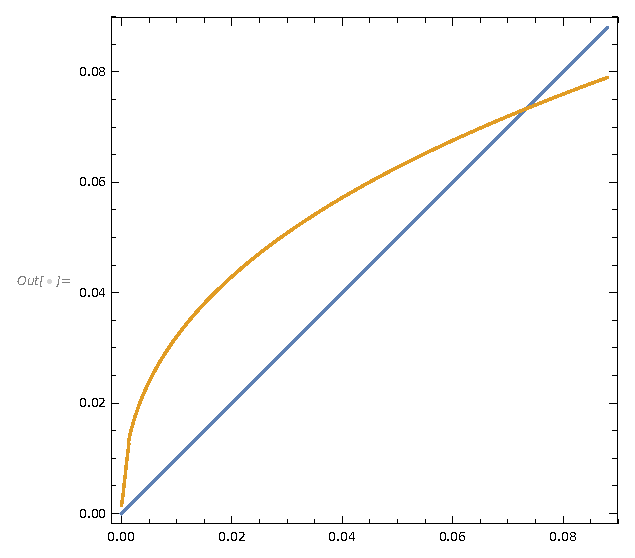
\includegraphics{xamples_gr1.eps}
\subsection*{Example 2}
Production function:    $f(k)=\frac{1}{\sqrt{0.5\, +\frac{0.5}{k^2}}}$

Utility function:       $u(c)=2 \sqrt{c}$

Savings function:       $s(w(k_t),f^\prime(k_{t+1}))= \frac{16. R w}{25.\, +16. R}$

Substituting:           $s(w(k_t),f^\prime(k_{t+1}))= \frac{8. \left(\frac{1}{\sqrt{0.5\, +\frac{0.5}{k^2}}}-\frac{0.5}{\left(0.5\, +\frac{0.5}{k^2}\right)^{3/2} k^2}\right)}{\left(25.\, +\frac{8.}{\left(0.5\, +\frac{0.5}{k^2}\right)^{3/2} k^3}\right) \left(0.5\, +\frac{0.5}{k^2}\right)^{3/2} k^3}$

Steady States:          Solve ${k}_{t+1}= \frac{1}{(1+n)}s(w(k_t),f^\prime(k_{t+1}))$

With the parameters: $\{k\to 0\}\}$

Stability:             Compute the derivative of $k_{t+1}$ with respect to $k_{t}$ and evaluate at each steady state.

With the parameters:

\quad Steady state 1, Capital level: $0$, Derivative=$0$. Stable.

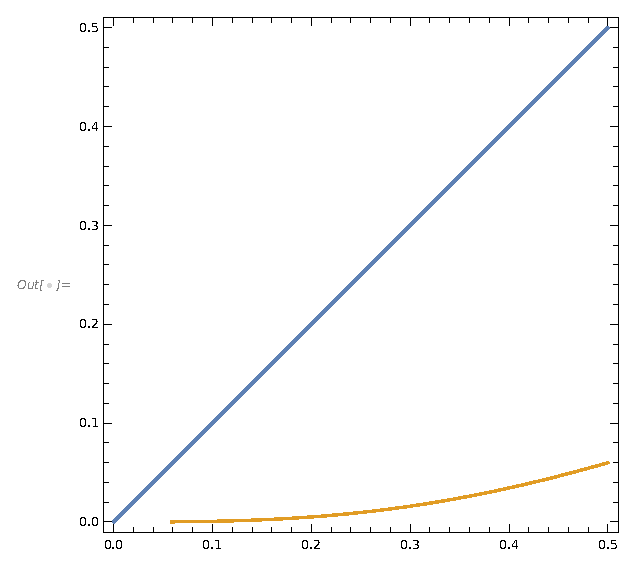
\includegraphics{xamples_gr2.eps}
\subsection*{Examples 3}
Production function:    $f(k)=\frac{1}{\sqrt{0.5\, +\frac{0.5}{k^2}}}$

Utility function:       $u(c)=\log(c)$

Savings function:       $s(w(k_t),f^\prime(k_{t+1}))= 0.444444 w$

Substituting: $s(w(k_t),f^\prime(k_{t+1}))= 0.444444 \left(\frac{1}{\sqrt{0.5\, +\frac{0.5}{k^2}}}-\frac{0.5}{\left(0.5\, +\frac{0.5}{k^2}\right)^{3/2} k^2}\right)$

Steady States:          Solve ${k}_{t+1}= \frac{1}{(1+n)}s(w(k_t),f^\prime(k_{t+1}))$

With the parameters: $\{k\to 0\}\}$

Stability:             Compute the derivative of $k_{t+1}$ with respect to $k_{t}$ and evaluate at each steady state.

With the parameters:

\quad Steady state 1, Capital level: $0$ Derivative=$0$. Stable.

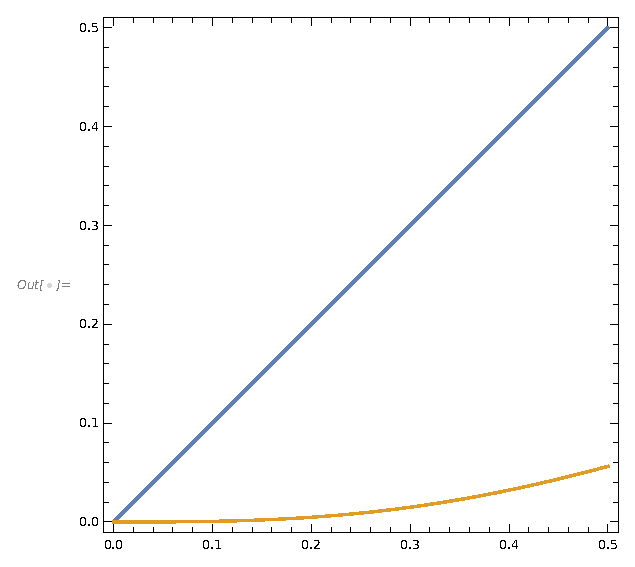
\includegraphics{xamples_gr3.eps}

\subsection*{Example 4}
Production function:    $f(k)=\left(0.5\, +0.5 k^{0.5}\right)^{2.}$

Utility function:       $u(c)log(c)$

Savings function:       $s(w(k_t),f^\prime(k_{t+1}))= 0.444444 w$

Substituting: $s(w(k_t),f^prime(k_{t+1}))= 0.444444 \left(\left(0.5\, +0.5 k^{0.5}\right)^{2.}-0.5 \left(0.5\, +0.5 k^{0.5}\right)^{1.} k^{0.5}\right)$

Steady States:          Solve ${k}_{t+1}= \frac{1}{(1+n)}s(w(k_t),f^\prime(k_{t+1}))$

With the parameters: $\{k\to 0.154832\}\}$

Stability:             Compute the derivative of $k_{t+1}$ with respect to $k_{t}$ and evaluate at each steady state.

With the parameters:

\quad Steady state 1, Capital level: $0.154832$ Derivative=$0.141188$  Stable.

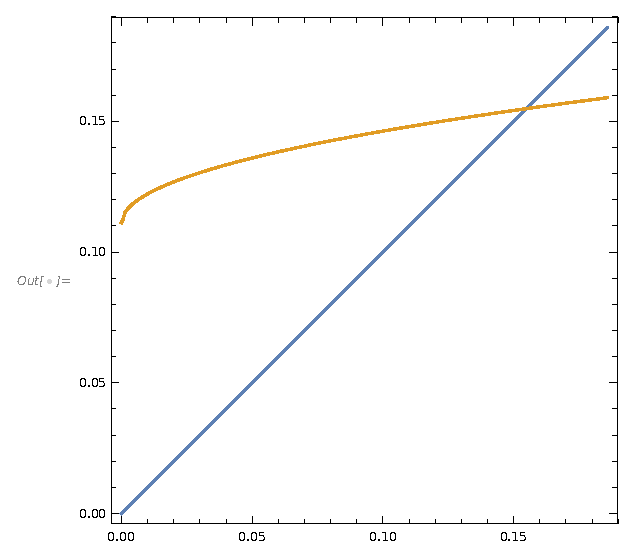
\includegraphics{xamples_gr4.eps}

\subsection*{Example 5}
Production function:    $f(k)=\left(0.5\, +0.5 k^{0.5}\right)^{2.}$

Utility function:       $u(c)=2 \sqrt{c}$

Savings function:       $s(w(k_t),f^\prime(k_{t+1}))= \frac{16. R w}{25.\, +16. R}$

Substituting:           $s(w(k_t),f^\prime(k_{t+1}))= \frac{\left(8. \left(0.5\, +0.5 k^{0.5}\right)^{1.} \left(\left(0.5\, +0.5 k^{0.5}\right)^{2.}-0.5 \left(0.5\, +0.5 k^{0.5}\right)^{1.} k^{0.5}\right)\right)}{\left(\left(25.\, +\frac{8. \left(0.5\, +0.5 k^{0.5}\right)^{1.}}{k^{0.5}}\right) k^{0.5}\right)}$

Steady States:          Solve ${k}_{t+1}= \frac{1}{(1+n)}s(w(k_t),f^\prime(k_{t+1}))$

With the parameters: $\{k\to 0.128222\}$

Stability:             Compute the derivative of $k_{t+1}$ with respect to $k_{t}$ and evaluate at each steady state.
With the parameters:

\quad Steady state 1, Capital level: $0.128222$ Derivative=$0.107258$ Stable.

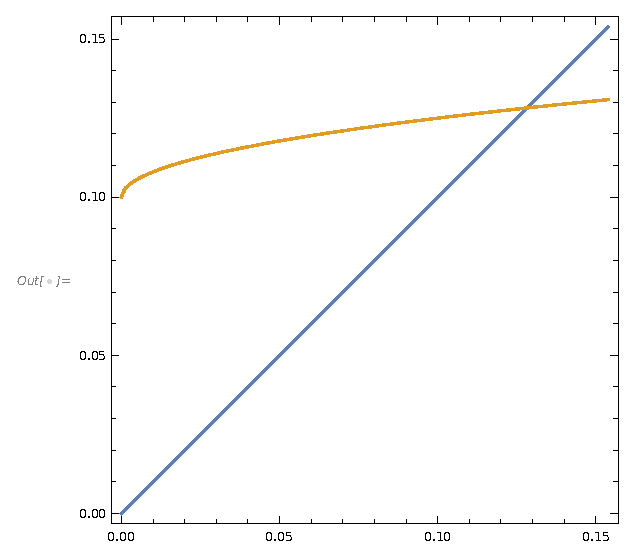
\includegraphics{xamples_gr5.eps}


\subsection*{Example 6}
Production function:    $f(k)=k^{0.5}$

Utility function:       $u(c)=\log(c)$

Savings function:       $s(w(k_t),f^\prime(k_{t+1}))= 0.444444 w$

Substituting:      $s(w(k_t),if^\prime(k_{t+1}))= 0.222222 k^{0.5}$

Steady States:          Solve ${k}_{t+1}= \frac{1}{(1+n)}s(w(k_t),f^\prime(k_{t+1}))$

With the parameters: $\{k\to 0.\},\{k\to 0.0493827\}$

Stability:             Compute the derivative of $k_{t+1}$ with respect to $k_{t}$ and evaluate at each steady state.

With the parameters:

\quad Steady state 1, Capital level: $0$. Derivative=$\infty$ Unstable.

\quad Steady state 2, Capital level: $0.0493827$ Derivative=$0.5$ Stable.

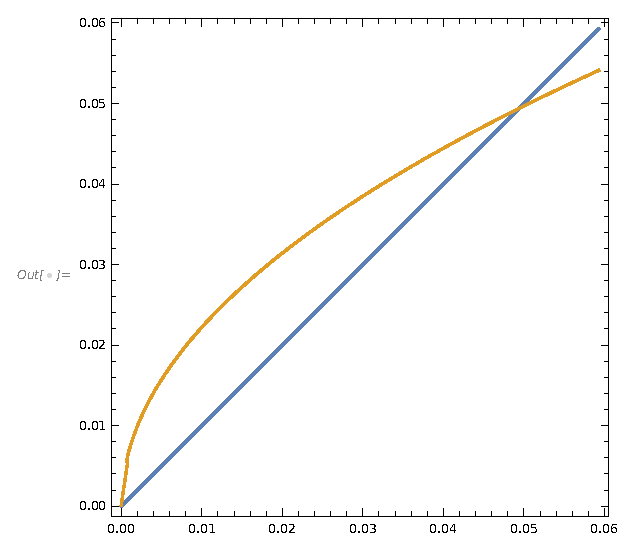
\includegraphics{xamples_gr6.eps}

\subsection*{Example 7}
Production function:    $f(k)=\frac{1}{0.9\, +\frac{0.1}{k}}$

Utility function:       $u(c)=2 \sqrt{c}$

Savings function:       $s(w(k_t),f^\prime(k_{t+1}))= \frac{16. R w}{25.\, +16. R}$

Substituting:           $s(w(k_t),f^\prime(k_{t+1})= \frac{1.6 \left(\frac{1}{0.9\, +\frac{0.1}{k}}-\frac{0.1}{\left(0.9\, +\frac{0.1}{k}\right)^2 k}\right)}{\left(25.\, +\frac{1.6}{\left(0.9\, +\frac{0.1}{k}\right)^2 k^2}\right) \left(0.9\, +\frac{0.1}{k}\right)^2 k^2}$

Steady States:          Solve ${k}_{t+1}= \frac{1}{(1+n)}s(w(k_t),f^\prime(k_{t+1}))$

With the parameters: $\{k\to 0.018251\},\{k\to 0.206304\}$

Stability:             Compute the derivative of $k_{t+1}$ with respect to $k_{t}$ and evaluate at each steady state.

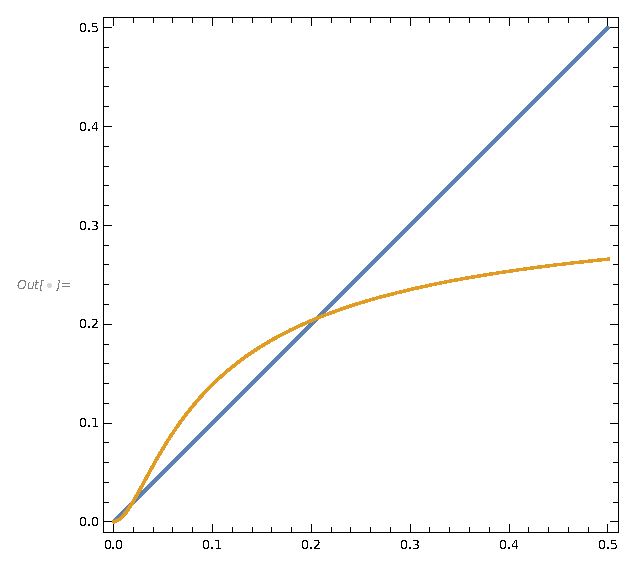
\includegraphics{xamples_gr7.eps}

\end{document}
